\documentclass{standalone}
\usepackage{tikz}
\usetikzlibrary{patterns, positioning}


\begin{document}
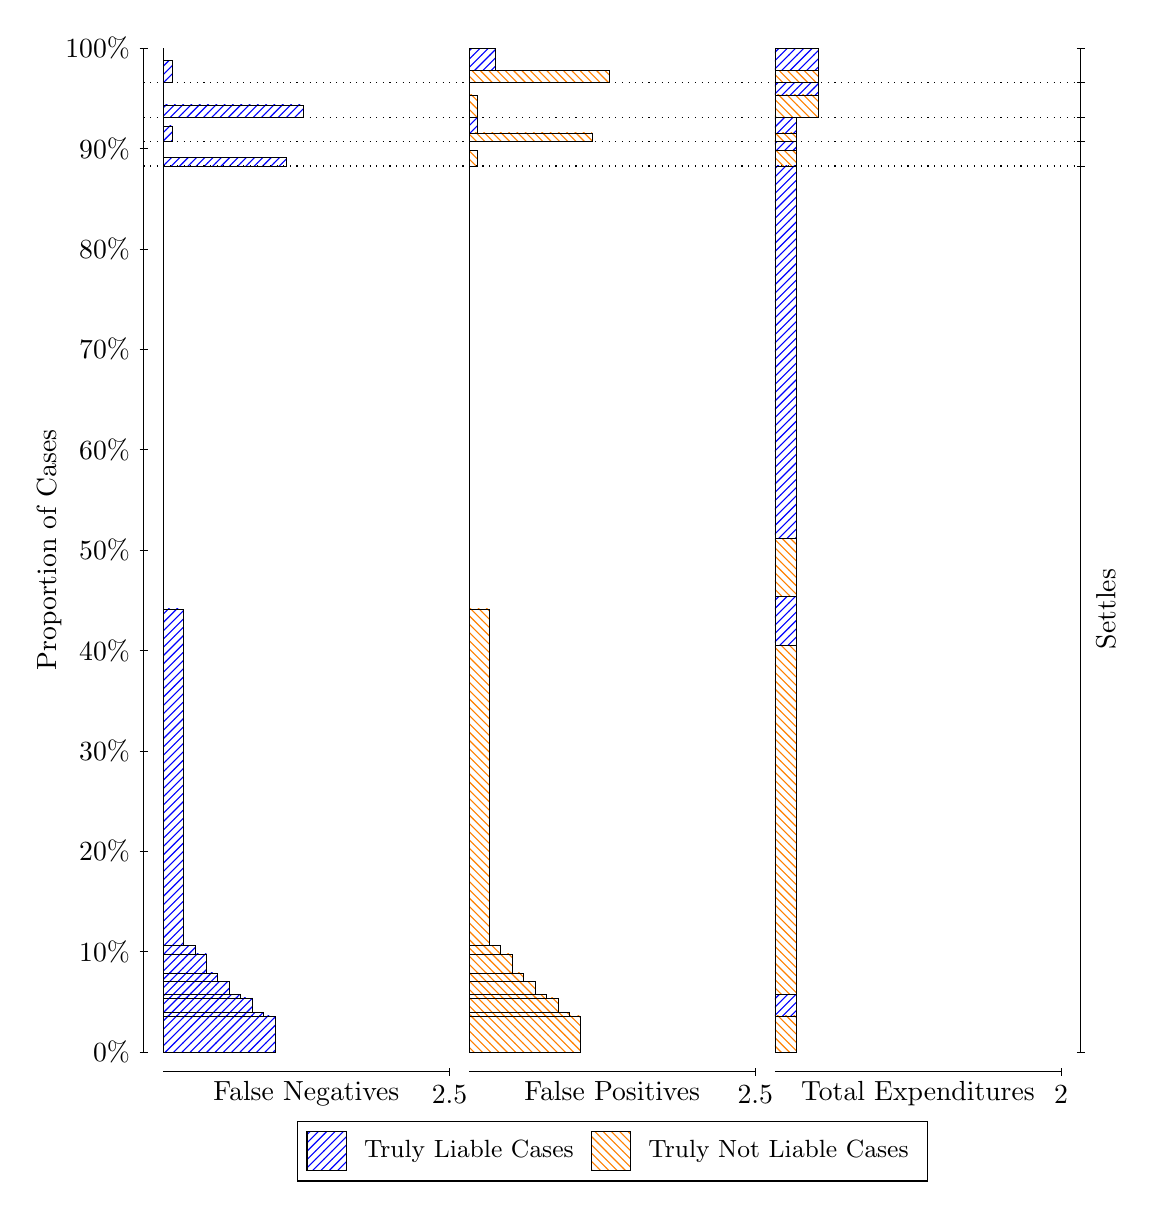
\begin{tikzpicture}
\draw[black, very thin] (1.5,1.75) -- (1.5,14.5);
\node[rotate=90, text=black, anchor=center] at (0.3, 8.125) {Proportion of Cases};
\draw[black, very thin] (1.45,1.75) -- (1.55,1.75);
\node[text=black, anchor=east] at (1.45, 1.75) {0\%};
\draw[black, very thin] (1.45,3.025) -- (1.55,3.025);
\node[text=black, anchor=east] at (1.45, 3.025) {10\%};
\draw[black, very thin] (1.45,4.3) -- (1.55,4.3);
\node[text=black, anchor=east] at (1.45, 4.3) {20\%};
\draw[black, very thin] (1.45,5.575) -- (1.55,5.575);
\node[text=black, anchor=east] at (1.45, 5.575) {30\%};
\draw[black, very thin] (1.45,6.85) -- (1.55,6.85);
\node[text=black, anchor=east] at (1.45, 6.85) {40\%};
\draw[black, very thin] (1.45,8.125) -- (1.55,8.125);
\node[text=black, anchor=east] at (1.45, 8.125) {50\%};
\draw[black, very thin] (1.45,9.4) -- (1.55,9.4);
\node[text=black, anchor=east] at (1.45, 9.4) {60\%};
\draw[black, very thin] (1.45,10.675) -- (1.55,10.675);
\node[text=black, anchor=east] at (1.45, 10.675) {70\%};
\draw[black, very thin] (1.45,11.95) -- (1.55,11.95);
\node[text=black, anchor=east] at (1.45, 11.95) {80\%};
\draw[black, very thin] (1.45,13.225) -- (1.55,13.225);
\node[text=black, anchor=east] at (1.45, 13.225) {90\%};
\draw[black, very thin] (1.45,14.5) -- (1.55,14.5);
\node[text=black, anchor=east] at (1.45, 14.5) {100\%};

\draw[black, very thin] (13.4,1.75) -- (13.4,14.5);
\draw[black, very thin] (13.35,1.75) -- (13.45,1.75);
\node[anchor=west] at (13.35, 1.75) {};
\draw[black, very thin] (13.35,13.002) -- (13.45,13.002);
\node[anchor=west] at (13.35, 13.002) {};
\draw[black, very thin] (13.35,13.312) -- (13.45,13.312);
\node[anchor=west] at (13.35, 13.312) {};
\draw[black, very thin] (13.35,13.622) -- (13.45,13.622);
\node[anchor=west] at (13.35, 13.622) {};
\draw[black, very thin] (13.35,14.061) -- (13.45,14.061);
\node[anchor=west] at (13.35, 14.061) {};
\draw[black, very thin] (13.35,14.5) -- (13.45,14.5);
\node[anchor=west] at (13.35, 14.5) {};

\draw[black, very thin, pattern color=blue, pattern=north east lines] (1.75,1.75) rectangle (3.167,2.2094);
\draw[black, very thin, pattern color=blue, pattern=north east lines] (1.75,2.2094) rectangle (3.0217,2.2573);
\draw[black, very thin, pattern color=blue, pattern=north east lines] (1.75,2.2573) rectangle (2.8763,2.4371);
\draw[black, very thin, pattern color=blue, pattern=north east lines] (1.75,2.4371) rectangle (2.731,2.485);
\draw[black, very thin, pattern color=blue, pattern=north east lines] (1.75,2.485) rectangle (2.5857,2.6464);
\draw[black, very thin, pattern color=blue, pattern=north east lines] (1.75,2.6464) rectangle (2.4403,2.7551);
\draw[black, very thin, pattern color=blue, pattern=north east lines] (1.75,2.7551) rectangle (2.295,2.9955);
\draw[black, very thin, pattern color=blue, pattern=north east lines] (1.75,2.9955) rectangle (2.1497,3.1042);
\draw[black, very thin, pattern color=blue, pattern=north east lines] (1.75,3.1042) rectangle (2.0043,7.376);
\draw[black, very thin, pattern color=orange, pattern=north west lines] (1.75,7.376) rectangle (1.75,13.002);
\draw[black, very thin, pattern color=blue, pattern=north east lines] (1.75,13.002) rectangle (3.3123,13.111);
\draw[black, very thin, pattern color=orange, pattern=north west lines] (1.75,13.111) rectangle (1.75,13.312);
\draw[black, very thin, pattern color=blue, pattern=north east lines] (1.75,13.312) rectangle (1.859,13.512);
\draw[black, very thin, pattern color=orange, pattern=north west lines] (1.75,13.512) rectangle (1.75,13.622);
\draw[black, very thin, pattern color=blue, pattern=north east lines] (1.75,13.622) rectangle (3.5303,13.777);
\draw[black, very thin, pattern color=orange, pattern=north west lines] (1.75,13.777) rectangle (1.75,14.061);
\draw[black, very thin, pattern color=blue, pattern=north east lines] (1.75,14.061) rectangle (1.859,14.344);
\draw[black, very thin, pattern color=orange, pattern=north west lines] (1.75,14.344) rectangle (1.75,14.5);
\draw[black, very thin, pattern color=orange, pattern=north west lines] (5.6333,1.75) rectangle (7.0503,2.2094);
\draw[black, very thin, pattern color=orange, pattern=north west lines] (5.6333,2.2094) rectangle (6.905,2.2573);
\draw[black, very thin, pattern color=orange, pattern=north west lines] (5.6333,2.2573) rectangle (6.7597,2.4371);
\draw[black, very thin, pattern color=orange, pattern=north west lines] (5.6333,2.4371) rectangle (6.6143,2.485);
\draw[black, very thin, pattern color=orange, pattern=north west lines] (5.6333,2.485) rectangle (6.469,2.6464);
\draw[black, very thin, pattern color=orange, pattern=north west lines] (5.6333,2.6464) rectangle (6.3237,2.7551);
\draw[black, very thin, pattern color=orange, pattern=north west lines] (5.6333,2.7551) rectangle (6.1783,2.9955);
\draw[black, very thin, pattern color=orange, pattern=north west lines] (5.6333,2.9955) rectangle (6.033,3.1042);
\draw[black, very thin, pattern color=orange, pattern=north west lines] (5.6333,3.1042) rectangle (5.8877,7.3759);
\draw[black, very thin, pattern color=blue, pattern=north east lines] (5.6333,7.3759) rectangle (5.6333,13.002);
\draw[black, very thin, pattern color=orange, pattern=north west lines] (5.6333,13.002) rectangle (5.7423,13.203);
\draw[black, very thin, pattern color=blue, pattern=north east lines] (5.6333,13.203) rectangle (5.6333,13.312);
\draw[black, very thin, pattern color=orange, pattern=north west lines] (5.6333,13.312) rectangle (7.1957,13.421);
\draw[black, very thin, pattern color=blue, pattern=north east lines] (5.6333,13.421) rectangle (5.7423,13.622);
\draw[black, very thin, pattern color=orange, pattern=north west lines] (5.6333,13.622) rectangle (5.7423,13.905);
\draw[black, very thin, pattern color=blue, pattern=north east lines] (5.6333,13.905) rectangle (5.6333,14.061);
\draw[black, very thin, pattern color=orange, pattern=north west lines] (5.6333,14.061) rectangle (7.4137,14.217);
\draw[black, very thin, pattern color=blue, pattern=north east lines] (5.6333,14.217) rectangle (5.9603,14.5);
\draw[black, very thin, pattern color=orange, pattern=north west lines] (9.5167,1.75) rectangle (9.7892,2.2078);
\draw[black, very thin, pattern color=blue, pattern=north east lines] (9.5167,2.2078) rectangle (9.7892,2.4833);
\draw[black, very thin, pattern color=orange, pattern=north west lines] (9.5167,2.4833) rectangle (9.7892,6.9165);
\draw[black, very thin, pattern color=blue, pattern=north east lines] (9.5167,6.9165) rectangle (9.7892,7.5373);
\draw[black, very thin, pattern color=orange, pattern=north west lines] (9.5167,7.5373) rectangle (9.7892,8.2723);
\draw[black, very thin, pattern color=blue, pattern=north east lines] (9.5167,8.2723) rectangle (9.7892,13.002);
\draw[black, very thin, pattern color=orange, pattern=north west lines] (9.5167,13.002) rectangle (9.7892,13.203);
\draw[black, very thin, pattern color=blue, pattern=north east lines] (9.5167,13.203) rectangle (9.7892,13.312);
\draw[black, very thin, pattern color=orange, pattern=north west lines] (9.5167,13.312) rectangle (9.7892,13.421);
\draw[black, very thin, pattern color=blue, pattern=north east lines] (9.5167,13.421) rectangle (9.7892,13.622);
\draw[black, very thin, pattern color=orange, pattern=north west lines] (9.5167,13.622) rectangle (10.062,13.905);
\draw[black, very thin, pattern color=blue, pattern=north east lines] (9.5167,13.905) rectangle (10.062,14.061);
\draw[black, very thin, pattern color=orange, pattern=north west lines] (9.5167,14.061) rectangle (10.062,14.217);
\draw[black, very thin, pattern color=blue, pattern=north east lines] (9.5167,14.217) rectangle (10.062,14.5);
\draw[black, dotted] (1.5,13.002) -- (13.4,13.002);
\draw[black, dotted] (1.5,13.312) -- (13.4,13.312);
\draw[black, dotted] (1.5,13.622) -- (13.4,13.622);
\draw[black, dotted] (1.5,14.061) -- (13.4,14.061);
\draw[black, very thin] (1.75,1.5) -- (5.3833,1.5);
\node[text=black, anchor=north] at (3.5667, 1.5) {False Negatives};
\draw[black, very thin] (5.3833,1.45) -- (5.3833,1.55);
\node[text=black, anchor=north] at (5.3833, 1.45) {2.5};

\draw[black, very thin] (5.6333,1.5) -- (9.2667,1.5);
\node[text=black, anchor=north] at (7.45, 1.5) {False Positives};
\draw[black, very thin] (9.2667,1.45) -- (9.2667,1.55);
\node[text=black, anchor=north] at (9.2667, 1.45) {2.5};

\draw[black, very thin] (9.5167,1.5) -- (13.15,1.5);
\node[text=black, anchor=north] at (11.333, 1.5) {Total Expenditures};
\draw[black, very thin] (13.15,1.45) -- (13.15,1.55);
\node[text=black, anchor=north] at (13.15, 1.45) {2};

\node[text=black, centered, rotate=90] at (13.72, 7.376) {Settles};





\draw (7.449999999999999,1.5) node[draw=none] (baseCoordinate) {};
\begin{scope}[align=center]
        \matrix[scale=0.5, draw=black, below=0.5cm of baseCoordinate, nodes={draw}, column sep=0.1cm]{
            \node[rectangle, draw, minimum width=0.5cm, minimum height=0.5cm, pattern color=blue, pattern=north east lines] {}; &
            \node[draw=none, font=\small, text=black] (B) {Truly Liable Cases}; &
            \node[rectangle, draw, minimum width=0.5cm, minimum height=0.5cm, pattern color=orange, pattern=north west lines] {}; &
            \node[draw=none, font=\small, text=black] (B) {Truly Not Liable Cases}; \\
            };
\end{scope}

\end{tikzpicture}
\end{document}